\documentclass[a4paper, 14pt]{article}
\usepackage[T2A]{fontenc}
\usepackage[utf8]{inputenc}
\usepackage[english,russian]{babel}
\usepackage[top = 2cm, bottom = 2 cm]{geometry}
\usepackage{cmap}
\usepackage{graphicx}
\usepackage{listings}
\usepackage{color}
\usepackage{amsmath}
\usepackage{pgfplots}
\usepackage{url}
\usepackage{tikz}
\usepackage{float}
\usepackage{multirow}
\usepackage{indentfirst}

\usepackage{titlesec}
\titleformat*{\section}{\LARGE\bfseries}
\titleformat*{\subsection}{\Large\bfseries}
\titleformat*{\subsubsection}{\large\bfseries}
\titleformat*{\paragraph}{\large\bfseries}
\titleformat*{\subparagraph}{\large\bfseries}


\begin{document}

	\textbf{Цель работы:} для сложной системы S, имеющей не более 10 состояний, определить  время нахождения системы в предельных состояниях, т.е. при установившемся режиме работы. 
	
	
	\section*{Теоретическая часть}
	
Случайный процесс, протекающий в сложной системе $S$, называется марковским, если он обладает следующим свойством:  для каждого момента времени $t_0$ вероятность любого состояния системы в будущем при $t > t_0$ зависит только от состояния системы в настоящем $t = t_0$ и не зависит от того, когда и каким образом система перешла в это состояние (как процесс развивался в прошлом). В марковском случайном процессе будущее развитие зависит только от настоящего состояния и не зависит от предыстории процесса.

Для марковского процесса составлены уравнения Колмогорова:
$$F=(P'(t), P(t), \lambda)=0$$


Вероятностью $i$-го состояния называется вероятность $p_i(t)$ того, что в момент времени $t$ система будет находиться в состоянии $S_i$. Для любого момента $t$ сумма вероятностей всех состояний равна единице. 

Для нахождения предельных вероятностей используется система уравнений вида:

\begin{equation*}
 \begin{cases}
   p'_0 = \lambda_{10}p_1 + \lambda_{20}p_2 - (\lambda_{01} + \lambda_{02})p_0,
   \\
  p'_1 = \lambda_{01}p_0 + \lambda_{31}p_3 - (\lambda_{10} + \lambda_{13})p_1,
   \\
  p'_2 = \lambda_{02}p_0 + \lambda_{32}p_3 - (\lambda_{20} + \lambda_{23})p_2,
  \\
  p'_3 = \lambda_{13}p_1 + \lambda_{23}p_2 - (\lambda_{31} + \lambda_{32})p_3.
 \end{cases}
\end{equation*}

В левой части каждого из уравнений стоит производная вероятности $i$-го состояния; в правой части - сумма произведений вероятностей всех состояний (из которых идут стрелки в данное состояние), умноженная на интенсивности соответствующих потоков событий, минус суммарная интенсивность всех потоков, выводящих систему из данного состояния, умноженная на вероятность данного $i$-го состояния.

\section*{Результаты работы}

На рис. \ref{fig:4} и  \ref{fig:10} представлены результаты работы программы:

\begin{figure}[H]
    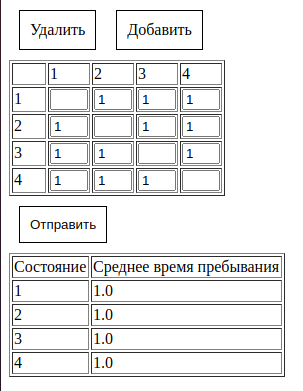
\includegraphics[scale=0.7]{4}
    \caption{Система S с 4 состояниями}
    \label{fig:4}
\end{figure}

\begin{figure}[H]
    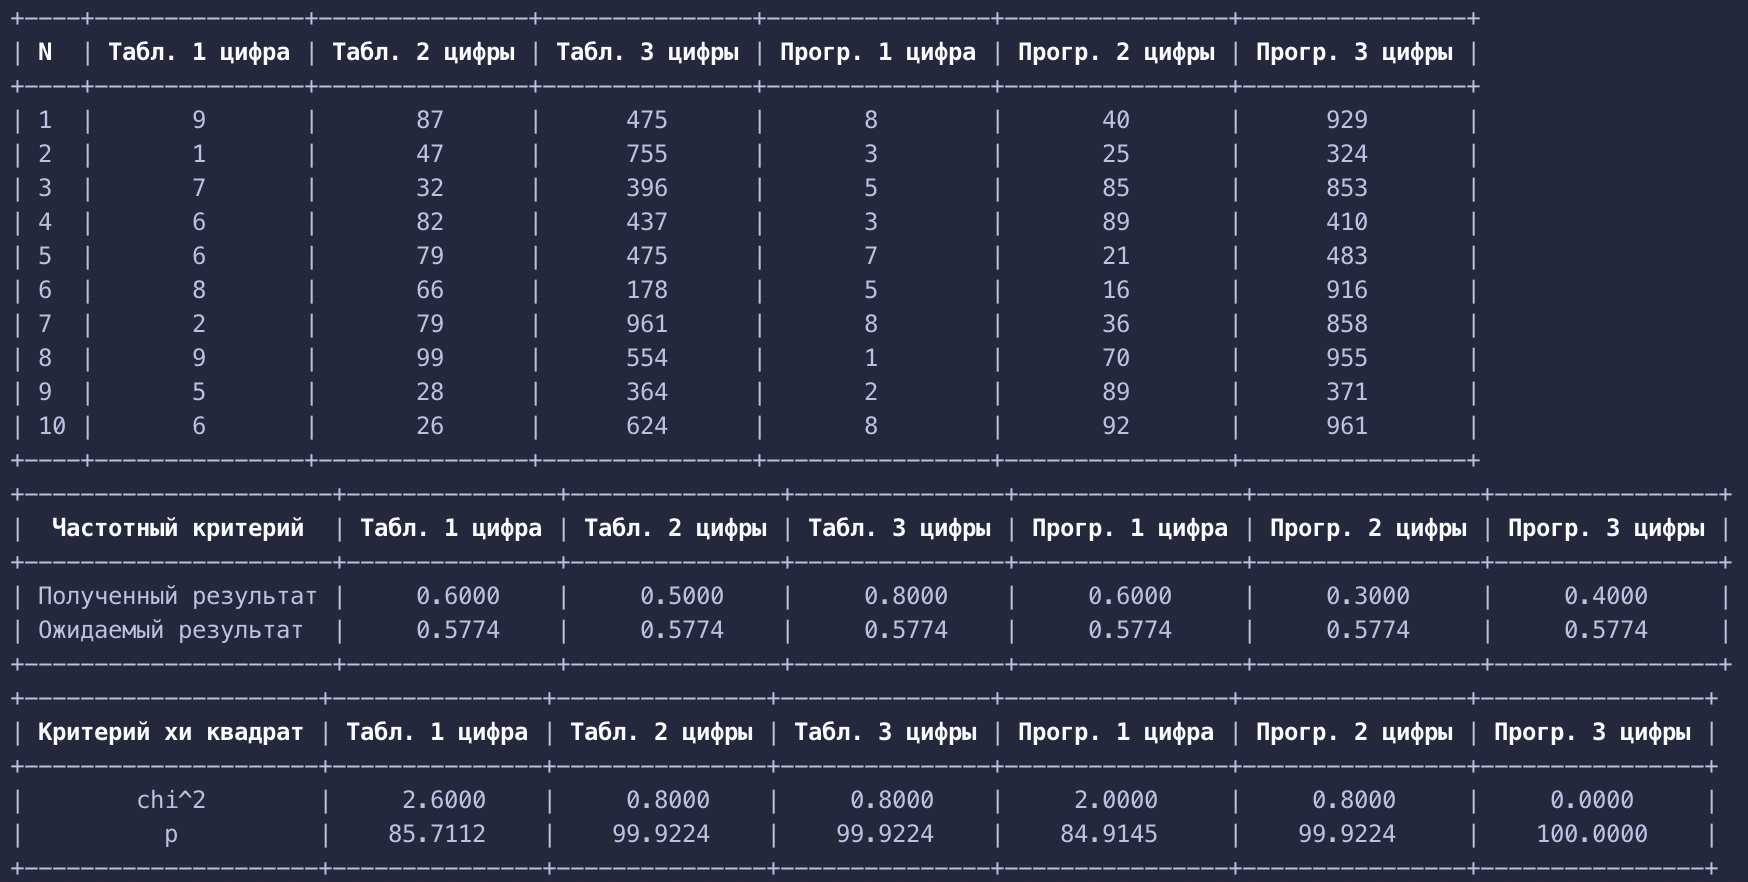
\includegraphics[scale=0.6]{10}
    \caption{Система S с 10 состояниями}
    \label{fig:10}
\end{figure}

\section*{Вывод}
В ходе выполнения лабораторной работы был смоделирован марковский процесс, найдены предельные вероятности и время нахождения сложной системы в передельных состояниях.
\end{document}